\documentclass[11pt,a4paper]{article}
% Közös preambulum a kézikönyvhöz és a programfelépítéshez
\usepackage[utf8]{inputenc}
\usepackage[T1]{fontenc}
\usepackage[magyar]{babel}
\usepackage{lmodern}
\usepackage{microtype}
\usepackage[a4paper,margin=2.3cm]{geometry}
\usepackage{graphicx}
\usepackage{booktabs,array,longtable,tabularx}
\usepackage{xcolor}
\usepackage{listings}
\usepackage{amsmath,amssymb}
\usepackage{textcomp}
\usepackage{csquotes}
\usepackage{enumitem}
\usepackage{caption}
\usepackage[most]{tcolorbox}
\usepackage{tikz}
\usetikzlibrary{arrows.meta,positioning,shapes.geometric,fit,calc,backgrounds}
\usepackage[hidelinks]{hyperref}

\graphicspath{{../img/}}
\newcommand{\rootdir}{../../..}
\setlist{itemsep=2pt,topsep=4pt}
\setlength{\parindent}{0pt}
\setlength{\parskip}{5pt}

\definecolor{kodhatter}{RGB}{247,247,247}
\definecolor{kulcsszo}{RGB}{0,0,150}
\definecolor{komment}{RGB}{0,115,0}
\definecolor{sztring}{RGB}{155,35,35}
\definecolor{fokek}{RGB}{31,90,160}
\definecolor{zold}{RGB}{44,160,44}
\definecolor{sarga}{RGB}{255,191,0}
\definecolor{narancs}{RGB}{255,127,14}
\definecolor{piros}{RGB}{214,39,40}

\newcommand{\kod}[1]{\texttt{#1}}

\lstset{
  language=Python,
  basicstyle=\ttfamily\small,
  backgroundcolor=\color{kodhatter},
  keywordstyle=\color{kulcsszo}\bfseries,
  commentstyle=\color{komment}\itshape,
  stringstyle=\color{sztring},
  breaklines=true, columns=fullflexible, keepspaces=true,
  showstringspaces=false, frame=single, rulecolor=\color{gray!35},
  framesep=4pt, xleftmargin=4pt, xrightmargin=4pt,
  tabsize=4, upquote=true,
  literate=
    {á}{{\'a}}1 {é}{{\'e}}1 {í}{{\'i}}1 {ó}{{\'o}}1 {ú}{{\'u}}1
    {Á}{{\'A}}1 {É}{{\'E}}1 {Í}{{\'I}}1 {Ó}{{\'O}}1 {Ú}{{\'U}}1
    {ö}{{\"o}}1 {ü}{{\"u}}1 {ő}{{\H{o}}}1 {ű}{{\H{u}}}1
    {Ö}{{\"O}}1 {Ü}{{\"U}}1 {Ő}{{\H{O}}}1 {Ű}{{\H{U}}}1
    {→}{{$\rightarrow$}}1 {←}{{$\leftarrow$}}1 {–}{{--}}1 {—}{{---}}1
    {·}{{$\cdot$}}1 {×}{{$\times$}}1 {±}{{$\pm$}}1 {≥}{{$\geq$}}1 {≤}{{$\leq$}}1
    {Σ}{{$\Sigma$}}1 {−}{{-}}1 {…}{{...}}1 {„}{{,,}}1 {”}{{''}}1
    {═}{{=}}1 {╦}{{+}}1 {║}{{|}}1 {─}{{-}}1 {│}{{|}}1
}
\lstdefinestyle{bash}{language=bash,keywordstyle=\color{black}}
\lstdefinestyle{lista}{basicstyle=\ttfamily\scriptsize,numbers=left,numberstyle=\tiny\color{gray},numbersep=5pt}

\newtcolorbox{megjegyzes}[1][Megjegyzés]{colback=fokek!5,colframe=fokek!70,fonttitle=\bfseries,title=#1,
  boxrule=0.6pt,arc=2pt,left=5pt,right=5pt,top=3pt,bottom=3pt}
\newtcolorbox{figyelem}[1][Figyelem]{colback=piros!4,colframe=piros!70,fonttitle=\bfseries,title=#1,
  boxrule=0.6pt,arc=2pt,left=5pt,right=5pt,top=3pt,bottom=3pt}


\title{\textbf{sumo\_morl}\\[6pt]
\Large Többcélú megerősítéses tanulás jelzőlámpa-vezérléshez\\[4pt]
\large Kézikönyv}
\date{}

\begin{document}
\maketitle
\thispagestyle{empty}

\begin{abstract}
\noindent A \kod{sumo\_morl} egy Python könyvtár, amellyel többcélú megerősítéses tanulással (MORL)
lehet jelzőlámpa-vezérlő ágenst fejleszteni a SUMO forgalomszimulátorban, forgalomtechnikai
előismeretek nélkül. A csomópont, a jelzésterv, a biztonsági (közbenső) idők, a detektorok és a
forgalom készen van; a feladat kizárólag az ágens megírása. Ez a kézikönyv elmagyarázza, mit
modellez a könyvtár, mit lát és mit csinálhat az ágens, mi alapján kap jutalmat, és hogyan érdemes
dolgozni vele. A programkód belső felépítését a \emph{Programfelépítés} dokumentum, az egyes
függvények és osztályok részletes leírását az \emph{API-referencia} (\kod{docs/sumo\_morl/api/index.html})
tartalmazza.
\end{abstract}

\tableofcontents
\newpage

%======================================================================
\section{Bevezetés}

\subsection{Mi a feladat?}

Egy jelzőlámpás csomópontban a vezérlő folyamatosan arról dönt, melyik irány kapjon zöldet. Egy
jó vezérlés kevés várakozással, kevés megállással és igazságosan szolgálja ki a járműveket.
Ezek a célok gyakran ellentmondanak egymásnak:

\begin{itemize}
  \item ha mindig a legtöbb járművet kiszolgáló irány kap zöldet, a kis forgalmú mellékág sokat vár;
  \item ha gyakran váltunk, mindenki hamar sorra kerül, de minden váltás néhány másodperc
        \enquote{elveszett időt} jelent (sárga, piros), ami csökkenti a csomópont áteresztőképességét.
\end{itemize}

Ezért nincs egyetlen legjobb vezérlés: csak \emph{kompromisszumok} vannak. A többcélú
megerősítéses tanulás (\emph{multi-objective reinforcement learning}, MORL) erre ad eszközöket: a
jutalom nem egy szám, hanem egy \textbf{vektor}, célonként egy elemmel, és a cél nem egyetlen ágens,
hanem a lehetséges kompromisszumok (a Pareto-front) feltérképezése.

\subsection{Mit ad a könyvtár, és mit kell megírni?}

\begin{center}
\begin{tabularx}{\linewidth}{@{}>{\raggedright\arraybackslash}X>{\raggedright\arraybackslash}X@{}}
\toprule
\textbf{Készen van} & \textbf{A hallgató feladata} \\
\midrule
T-csomópont hálózata a SUMO-ban & az ágens (pl. DQN, PPO, saját MORL algoritmus) \\
jelzőcsoportok, fázisok, biztonságos fázisátmenetek & a célfüggvények kiválasztása, esetleg saját cél \\
indukcióshurok-detektorok, mérések aggregálása & a tanítás és a kiértékelés megtervezése \\
véletlen, reális forgalmi igény & az eredmények (Pareto-front) elemzése \\
Gymnasium környezet vektor-jutalommal & \\
összehasonlító (klasszikus) vezérlők, MORL segédfüggvények, ábrák & \\
\bottomrule
\end{tabularx}
\end{center}

Az ágens minden döntési pontban \textbf{egyetlen dolgot} mond meg: melyik fázis legyen a
következő. A környezet gondoskodik róla, hogy a jelzőlámpák ezután szabályosan és biztonságosan
váltsanak.

\subsection{Alapfogalmak röviden}

\begin{description}[style=nextline,leftmargin=1.5em]
  \item[Ágens, környezet, lépés] Az ágens megfigyelést kap, akciót választ, a környezet szimulál egy
    darabig, majd új megfigyelést és jutalmat ad vissza. Egy \emph{epizód} egy szimulált időszak
    (alapértelmezés szerint egy óra).
  \item[Vektor-jutalom] Minden lépésben egy $k$ elemű vektor $\mathbf r_t = (r^1_t,\dots,r^k_t)$,
    ahol $k$ a célok száma. Az epizód vektor-hozama $\mathbf R = \sum_t \mathbf r_t$.
  \item[Dominancia, Pareto-front] Egy $\mathbf R_a$ hozam \emph{dominálja} $\mathbf R_b$-t, ha minden
    célban legalább olyan jó, és legalább egyben jobb. A nem dominált hozamok halmaza a
    \emph{Pareto-front}.
  \item[Skalarizálás] A vektor-jutalom egy számmá alakítása, pl. súlyozott összeggel:
    $r_t = \mathbf w^\top \mathbf r_t$, ahol $\mathbf w \geq 0$, $\sum_i w_i = 1$. Különböző súlyokkal
    a front különböző pontjai érhetők el.
\end{description}

%======================================================================
\section{Telepítés és első futtatás}

\subsection{Telepítés}

Python 3.9 vagy újabb kell. A csomag gyökérkönyvtárában (ahol a \kod{pyproject.toml} van):

\begin{lstlisting}[style=bash]
python -m venv .venv
source .venv/bin/activate        # Windows: .venv\Scripts\activate
pip install -e .                 # a könyvtár és a SUMO
pip install -e ".[rl]"           # opcionális: Stable-Baselines3 a tanítási példához
python -m pytest                 # ellenőrzés: a tesztek kb. fél perc alatt lefutnak
\end{lstlisting}

A SUMO-t az \kod{eclipse-sumo} pip csomag hozza magával, külön telepíteni nem kell. Ha a gépen már van
SUMO, és a \kod{SUMO\_HOME} környezeti változó be van állítva, a könyvtár azt használja.

\subsection{Demó: klasszikus fix idejű program}

Mielőtt bármilyen ágenst írnál, nézd meg a működést a legegyszerűbb vezérléssel. A fix idejű
program a fázisokat mindig ugyanabban a sorrendben, mindig ugyanannyi ideig tartja zölden
(alapértelmezés: 30, 10 és 15 másodperc), a forgalomtól függetlenül.

\begin{lstlisting}[style=bash]
python examples/sumo_morl/00_demo_fix_ido.py --gui              # SUMO grafikus felülettel
python examples/sumo_morl/00_demo_fix_ido.py --green 40 10 20   # más zöldidőkkel
\end{lstlisting}

A program először kiírja a fázisokat, a köztük lévő átmeneteket és a ciklusidőt (a ciklus egy teljes
kör az összes fázison; itt $30+4+10+5+15+5 = 69$~s). Ezután minden fázisváltásnál kiírja a
detektorokból becsült járműszámot ágankként, a végén pedig az epizód jutalmait és néhány valós
mutatót (átlagos késés, utazási idő). Elmenti az első két ciklus jelzéstervét is
(\ref{fig:jelzesterv}.~ábra).

\begin{figure}[h]
  \centering
  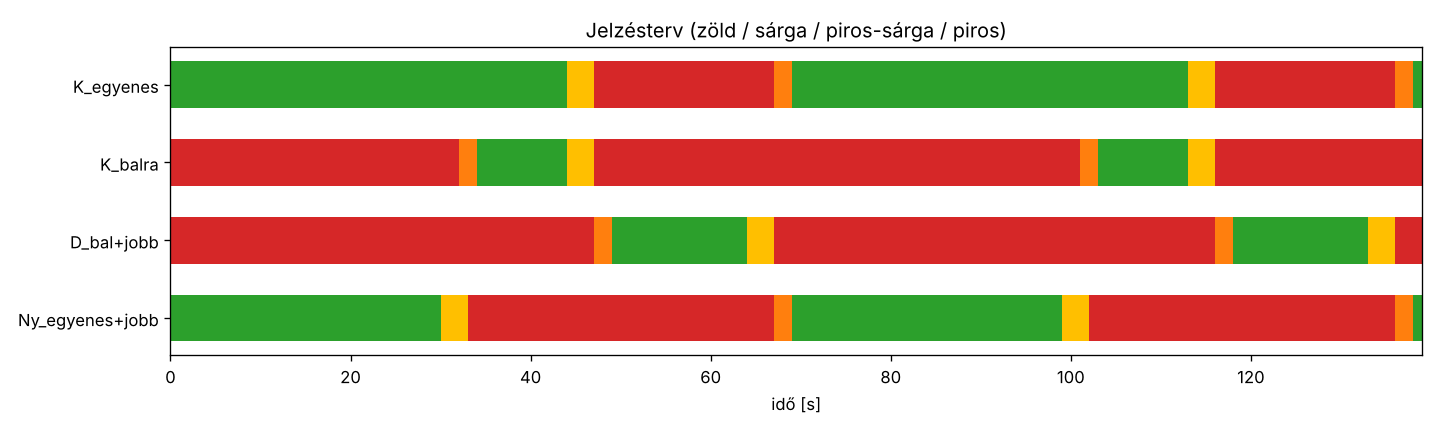
\includegraphics[width=\linewidth]{fix_ido_jelzesterv.png}
  \caption{A fix idejű program első két ciklusa jelzőcsoportonként. Zöld: szabad jelzés; sárga: a zöld
    vége; narancs: piros-sárga (indulás előtt); piros: tilos. A keleti egyenes sáv két egymást követő
    fázisban is zöld, ezért a zöldje hosszabb.}
  \label{fig:jelzesterv}
\end{figure}

\begin{megjegyzes}[Érdemes kipróbálni]
Futtasd a demót \kod{--gui} kapcsolóval, és figyeld meg a SUMO felületén a sárga és a piros-sárga
jelzéseket, a balra kanyarodók külön sávját, és azt, hogyan nő a sor a mellékágon, amíg piros.
Utána próbálj ki más zöldidőket, és figyeld, hogyan változnak a jutalmak.
\end{megjegyzes}

\subsection{A legkisebb saját program}

\begin{lstlisting}
import numpy as np
from sumo_morl import TJunctionMOEnv

env = TJunctionMOEnv(objectives=("queue", "fairness", "switches"))
obs, info = env.reset(seed=0)
R = np.zeros(env.reward_dim)
done = False
while not done:
    action = env.action_space.sample()     # ide kerül az ágens döntése
    obs, reward, terminated, truncated, info = env.step(action)
    R += reward                            # a reward egy vektor
    done = terminated or truncated
print(dict(zip(env.objective_names, R)))
env.close()
\end{lstlisting}

%======================================================================
\section{A szimulált csomópont}

\subsection{Geometria}

Egyszerű T-csomópont jobbkezes forgalommal (\ref{fig:csomopont}.~ábra). Mindhárom ág 250~m
hosszú, a megengedett sebesség 50~km/h. A főút nyugat--kelet irányú, a mellékág délről csatlakozik.

\begin{figure}[h]
  \centering
  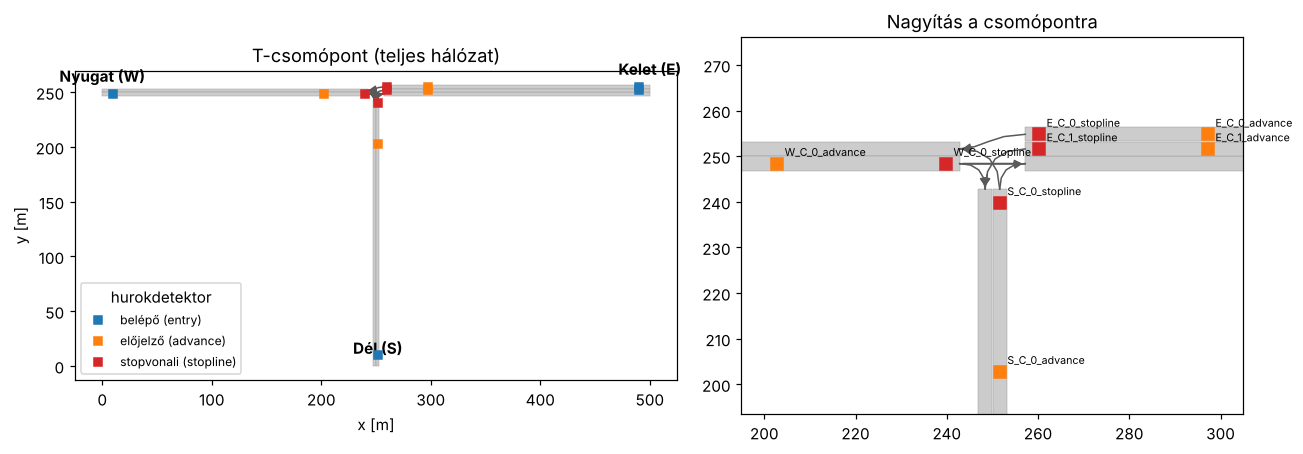
\includegraphics[width=\linewidth]{csomopont.png}
  \caption{A csomópont és a hurokdetektorok. Balra a teljes hálózat, jobbra nagyítás a csomópontra.}
  \label{fig:csomopont}
\end{figure}

\begin{center}
\begin{tabular}{@{}lll@{}}
\toprule
Ág & Bejövő sáv & Mozgások \\
\midrule
Nyugat (W) & \kod{W\_C\_0} & egyenesen keletre és jobbra délre (közös sáv) \\
Kelet (E)  & \kod{E\_C\_0} & egyenesen nyugatra \\
Kelet (E)  & \kod{E\_C\_1} & balra, délre (külön kanyarodósáv) \\
Dél (S)    & \kod{S\_C\_0} & balra nyugatra és jobbra keletre (közös sáv) \\
\bottomrule
\end{tabular}
\end{center}

A keleti bejövő ág tehát két sávra van osztva: a balra kanyarodók külön sávban várnak, így nem
tartják fel az egyenesen haladókat. Visszafordulás nincs.

\subsection{Jelzőcsoportok, konfliktusok és fázisok}

\begin{description}[style=nextline,leftmargin=1.5em]
  \item[Jelzőcsoport] Mozgások halmaza, amelyek mindig ugyanazt a jelzést kapják. Itt egy bejövő sáv
    egy jelzőcsoport, így négy csoport van: \kod{Ny\_egyenes+jobb}, \kod{K\_egyenes},
    \kod{K\_balra}, \kod{D\_bal+jobb}.
  \item[Konfliktus] Két csoport konfliktusos, ha járműveik útvonala keresztezi egymást vagy
    összefut. Konfliktusos csoportok nem kaphatnak egyszerre zöldet.
  \item[Fázis] Egymással nem konfliktusos csoportok halmaza, amelyek együtt kapnak zöldet.
\end{description}

A fázisokat a könyvtár a konfliktusokból számolja: a konfliktusmentes csoportok
\emph{maximális} halmazai lesznek a fázisok (gráfelméleti nyelven: a kompatibilitási gráf
klikkjei). Ebből a csomópontból pontosan három fázis adódik (\ref{fig:fazisok}.~ábra):

\begin{center}
\begin{tabular}{@{}cll@{}}
\toprule
Fázis & Zöldet kap & Leírás \\
\midrule
0 & \kod{W\_C\_0}, \kod{E\_C\_0} & főirány mindkét irányban egyenesen (és nyugatról jobbra) \\
1 & \kod{E\_C\_0}, \kod{E\_C\_1} & keleti ág: egyenes és védett balra kanyarodás \\
2 & \kod{S\_C\_0} & déli mellékág \\
\bottomrule
\end{tabular}
\end{center}

\begin{figure}[h]
  \centering
  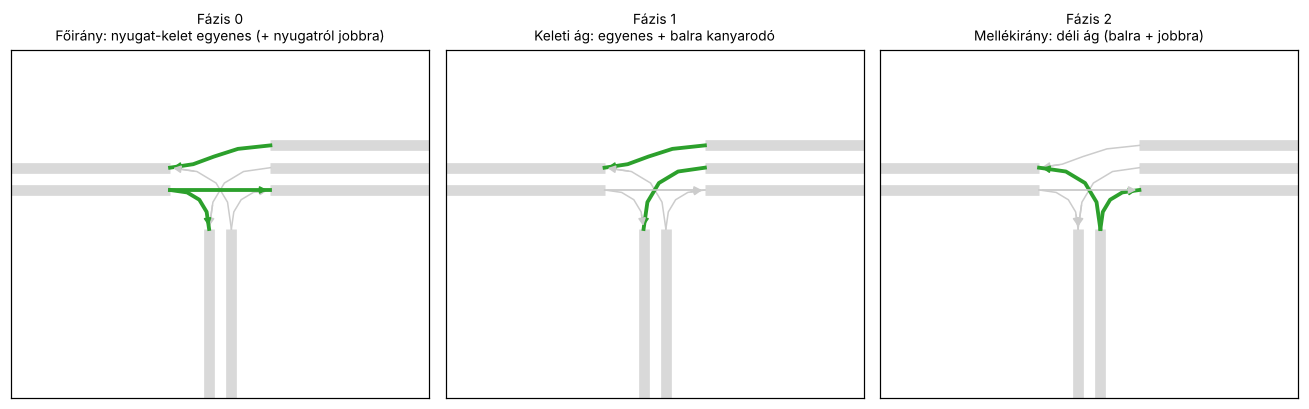
\includegraphics[width=\linewidth]{fazisok.png}
  \caption{A három fázis. Zölddel a szabad jelzést kapó mozgások.}
  \label{fig:fazisok}
\end{figure}

\subsection{Közbenső idők}

Amikor egy irány zöldje véget ér, az utolsó, még zölden behajtó jármű egy ideig a csomópontban
van. A vele konfliktusos irány csak akkor kaphat zöldet, amikor ez a jármű már biztosan elhagyta az
ütközési pontot. Az ehhez szükséges minimális időt nevezzük \textbf{közbenső időnek}
(\emph{intergreen}): $k(i\to j)$ az $i$ csoport zöldjének vége és a $j$ csoport zöldjének kezdete
között legalább eltelő idő.

A közbenső időket a mellékelt közbensőidő-számító kód (\kod{geometry\_utils.py},
\kod{sumo\_parser.py}) számolja a csomópont geometriájából:

\begin{enumerate}
  \item minden mozgás pályáját simított görbével közelíti, ebből kanyarodási sugarat, abból
        jellemző sebességet számol;
  \item megkeresi a pályák ütközési pontjait;
  \item minden ütközési pontra kiszámolja
  \[
    k = t_\text{át} + \frac{s_\text{ki} + l_\text{jármű}}{v_\text{ki}} - \frac{s_\text{be}}{v_\text{be}},
  \]
  ahol $t_\text{át}=3$~s, $l_\text{jármű}=6$~m, $s_\text{ki}$ a kiürítő jármű útja a stopvonaltól az
  ütközési pontig, $s_\text{be}$ a belépő jármű útja az ütközési pontig, $v_\text{ki}$ és
  $v_\text{be}$ a sebességeik. Az eredményt egész másodpercre felfelé kerekíti.
\end{enumerate}

A jelzőcsoportok közötti közbenső idő a csoportok mozgásai közötti értékek maximuma
(\ref{fig:kozbenso}.~ábra).

\begin{figure}[h]
  \centering
  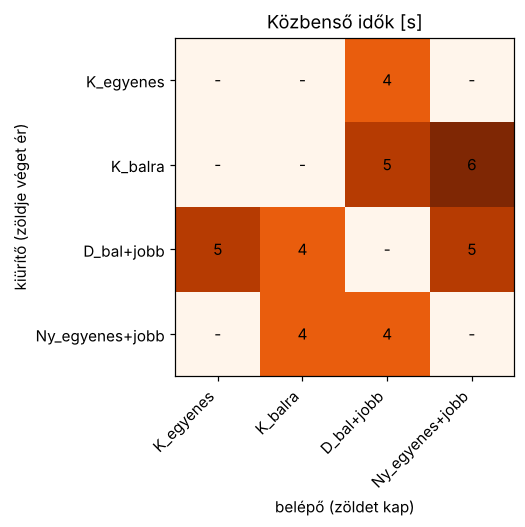
\includegraphics[width=0.48\linewidth]{kozbenso_idok.png}
  \caption{Közbenső idők [s] a jelzőcsoportok között. Sor: a csoport, amelynek a zöldje véget ér;
    oszlop: a csoport, amely zöldet kap; \enquote{--}: nincs konfliktus.}
  \label{fig:kozbenso}
\end{figure}

\subsection{Fázisátmenetek}

Fázisváltáskor a környezet automatikusan lejátssza az átmenetet:

\begin{itemize}
  \item a megszűnő csoportok 3~s \textcolor{sarga!80!black}{\textbf{sárgát}}, majd pirosat kapnak;
  \item az induló csoportok akkor kapnak zöldet, amikor a közbenső idők ezt megengedik (legalább 2~s
        után), előtte 2~s \textcolor{narancs}{\textbf{piros-sárgát}};
  \item a mindkét fázisban zöld csoportok végig zöldek maradnak.
\end{itemize}

Az átmenetek hossza másodpercben:

\begin{center}
\begin{tabular}{@{}c|ccc@{}}
honnan $\backslash$ hova & 0 & 1 & 2 \\
\midrule
0 & -- & 4 & 4 \\
1 & 6 & -- & 5 \\
2 & 5 & 5 & -- \\
\end{tabular}
\end{center}

\begin{megjegyzes}
Az átmenetek alatt egyik konfliktusos irány sem haladhat, ezért ez az idő a forgalom szempontjából
elveszett. Ez az egyik oka annak, hogy a túl gyakori váltás rossz.
\end{megjegyzes}

%======================================================================
\section{Hogyan vezérel az ágens?}

\subsection{Akciók}

Az akciótér \kod{Discrete(3)}: az akció a \textbf{következő fázis} sorszáma.

\begin{itemize}
  \item \textbf{Ha az akció az aktuális fázis}, a zöld \kod{decision\_interval} (alapértelmezés 5)
        másodperccel meghosszabbodik, utána jön a következő döntés.
  \item \textbf{Ha más fázist választ}, lefut a szabályos átmenet (4--6~s), majd az új fázis
        \kod{min\_green} (alapértelmezés 5) másodpercig biztosan zöld. Csak ezután jön a következő
        döntés.
\end{itemize}

Bármelyik akció mindig érvényes, szabálytalan jelzéskép nem állhat elő. Opcionálisan megadható egy
legnagyobb zöldidő (\kod{max\_green}); ha egy zöld ennél tovább tartana, a környezet kikényszeríti a
váltást a következő fázisra.

\begin{figure}[h]
\centering
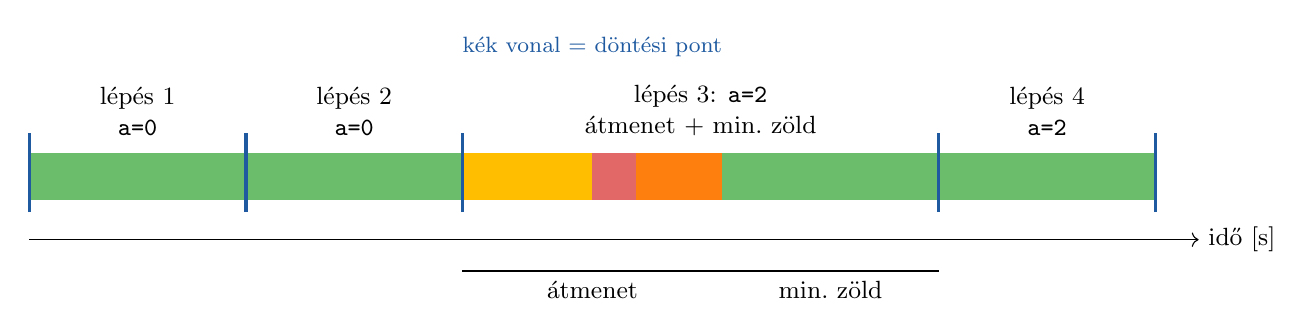
\begin{tikzpicture}[x=0.55cm,y=1cm,font=\small]
  \fill[zold!70] (0,0) rectangle (5,0.6);
  \fill[zold!70] (5,0) rectangle (10,0.6);
  \fill[sarga] (10,0) rectangle (13,0.6);
  \fill[piros!70] (13,0) rectangle (14,0.6);
  \fill[narancs] (14,0) rectangle (16,0.6);
  \fill[zold!70] (16,0) rectangle (21,0.6);
  \fill[zold!70] (21,0) rectangle (26,0.6);
  \foreach \x in {0,5,10,21,26} \draw[very thick,fokek] (\x,-0.15) -- (\x,0.85);
  \draw[->] (0,-0.5) -- (27,-0.5) node[right] {idő [s]};
  \node[above,align=center] at (2.5,0.7) {lépés 1\\\kod{a=0}};
  \node[above,align=center] at (7.5,0.7) {lépés 2\\\kod{a=0}};
  \node[above,align=center] at (15.5,0.7) {lépés 3: \kod{a=2}\\átmenet + min.\ zöld};
  \node[above,align=center] at (23.5,0.7) {lépés 4\\\kod{a=2}};
  \draw[thick] (10,-0.9) -- (16,-0.9) node[midway,below] {átmenet};
  \draw[thick] (16,-0.9) -- (21,-0.9) node[midway,below] {min.\ zöld};
  \node[fokek] at (13,1.95) {\footnotesize kék vonal = döntési pont};
\end{tikzpicture}
\caption{Döntési pontok az időben. Maradás esetén a lépés 5~s, váltáskor az átmenettel és a
  minimális zölddel együtt 9--11~s.}
\label{fig:lepesek}
\end{figure}

\subsection{Változó lépéshossz}

A \ref{fig:lepesek}.~ábrán látható, hogy a lépések hossza nem állandó. Az adott lépés hossza
másodpercben az \kod{info["elapsed"]} értékben található. A jutalmak a lépés másodperceire vannak
összegezve, így az epizód összjutalma a lépéshosszaktól függetlenül a teljes időre vett összeg. Ha
diszkontálva tanulsz, érdemes lehet a diszkontot a lépés hosszához igazítani
($\gamma^{\text{elapsed}}$); ez jó haladó feladat.

\subsection{Epizódok és forgalom}

Egy epizód alapértelmezés szerint 3600 szimulált másodperc. Minden \kod{reset()} új epizódot
indít új, véletlen forgalommal: a főirányon irányonként 200--700, a mellékágon 80--400 jármű óránként,
10--45\%-os kanyarodási arányokkal. A járművek véletlen időpontokban (Poisson-folyamat szerint)
érkeznek. Azonos \kod{seed} azonos forgalmat ad, így a vezérlők igazságosan összehasonlíthatók.

Rögzített igény is megadható:

\begin{lstlisting}
from sumo_morl import TJunctionMOEnv, Demand

env = TJunctionMOEnv(demand=Demand.constant(main=600, side=250))
env = TJunctionMOEnv(demand=lambda rng: Demand.random(rng, main_range=(400, 800)))
env.reset(options={"demand": Demand.constant(300, 100)})   # csak erre az epizódra
\end{lstlisting}

%======================================================================
\section{Mit lát az ágens?}

\subsection{Csak mérhető adatok}

Egy valódi csomópont vezérlője nem látja a járműveket: nem tudja, hány autó áll a sorban, ki mióta
vár vagy hová tart. Csak azt tudja, amit az úttestbe épített \textbf{indukcióshurok-detektorok}
mérnek. Ahhoz, hogy a tanult vezérlés a valóságba is átvihető legyen, a könyvtár megfigyelése és
jutalma \textbf{kizárólag ilyen mérhető adatokból} készül.

\subsection{A detektorok}

Minden bejövő sávon (összesen 4) három hurok van, így összesen 12:

\begin{center}
\begin{tabular}{@{}lll@{}}
\toprule
Típus & Helye & Mire jó \\
\midrule
belépő (\kod{entry})        & 10~m-re az ág elejétől & a csomópont felé érkező járművek számlálása \\
előjelző (\kod{advance})    & 40~m-re a stopvonaltól  & közeledő járművek; ha tartósan foglalt, a sor idáig ér \\
stopvonali (\kod{stopline}) & 3~m-re a stopvonaltól   & az áthaladó járművek számlálása, a sor eleje \\
\bottomrule
\end{tabular}
\end{center}

Egy hurok minden lépésben négy mennyiséget ad:

\begin{center}
\begin{tabular}{@{}lp{0.62\linewidth}@{}}
\toprule
\kod{count}     & a lépés alatt áthaladt járművek száma \\
\kod{occupancy} & foglaltság: az idő hányadában volt jármű a hurok felett (0--1) \\
\kod{speed}     & átlagsebesség a hurkon [m/s]; ha nem volt jármű, a megengedett sebesség \\
\kod{gap}       & a legutóbbi érzékelés óta eltelt idő [s] (időrés) \\
\bottomrule
\end{tabular}
\end{center}

\subsection{Becsült járműszám (bemenet--kimenet módszer)}

A belépő és a stopvonali hurok számlálóiból folyamatosan számolható, hány jármű van a kettő
között:
\[
  N(t) = N(t-1) + \text{belépők}(t) - \text{kilépők}(t).
\]
Ezt ágankként számoljuk (a keleti ág két sávját együtt, mert a járművek sávot válthatnak). A
tesztek szerint a becslés legfeljebb néhány járművel tér el a szimuláció valós értékétől.

\subsection{A megfigyelésvektor}

A megfigyelés egy 55 elemű, $[0,1]$ tartományba normalizált vektor:

\begin{center}
\begin{tabular}{@{}lrl@{}}
\toprule
Tartalom & Elemszám & Normalizálás \\
\midrule
detektoronként \kod{count}, \kod{occupancy}, \kod{speed}, \kod{gap} & $12\times4=48$ & lásd lent \\
becsült járműszám ágankként (W, E, S) & 3 & az ág tárolókapacitásához ($\approx$7~m/jármű) \\
aktuális fázis (one-hot) & 3 & 0 vagy 1 \\
az aktuális zöld eddigi hossza & 1 & /120~s \\
\bottomrule
\end{tabular}
\end{center}

A detektoradatok normalizálása: a forgalom (jármű/óra) 1800 jármű/órához, a sebesség a sebességkorláthoz,
az időrés 60~s-hoz viszonyítva, mindegyik 1-nél levágva. Az egyes elemek neve az
\kod{env.observation\_names()} függvénnyel kérdezhető le (pl. \kod{'E\_C\_1\_stopline.occupancy'}).

A nyers, aggregált detektoradatok az \kod{info["detectors"]} objektumban is elérhetők, így saját
megfigyelés is építhető (pl. \kod{gymnasium.ObservationWrapper}-rel).

\subsection{Amit szándékosan nem lát az ágens}

Jármű-azonosítók, pozíciók, úticélok, pontos sorhossz, várakozási idő, emisszió. Ezeket a környezet
az \kod{info["ground\_truth"]} alatt kiírja, de \textbf{csak kiértékeléshez}.

\begin{figyelem}[Ne csalj!]
Az \kod{info["ground\_truth"]} adatait (pl. átlagos késés, CO\textsubscript{2}) használd a
dolgozatban annak bemutatására, hogy a vezérlőd tényleg jobb. A megfigyelésbe vagy a jutalomba
viszont ne építsd be őket, mert a valóságban nem mérhetők.
\end{figyelem}

%======================================================================
\section{Mit tanul az ágens? -- célfüggvények}

\subsection{Vektor-jutalom}

A környezet létrehozásakor választod ki a célokat; a jutalomvektor ebben a sorrendben tartalmazza
őket:

\begin{lstlisting}
env = TJunctionMOEnv(objectives=("queue", "fairness", "switches"))  # alapértelmezés
env.objective_names        # ('queue', 'fairness', 'switches')
\end{lstlisting}

Konvenció: \textbf{nagyobb érték = jobb}, a költségek negatív előjelűek. Minden cél a lépés
másodperceire összegzett mennyiség, és egy rögzített skálával szorozva van, hogy a tipikus
lépésenkénti értékek 1 körüliek legyenek.

\begin{center}
\begin{tabularx}{\linewidth}{@{}l>{\raggedright\arraybackslash}X>{\raggedright\arraybackslash}X@{}}
\toprule
Név & Mit mér (lépésenként) & Mit jelent \\
\midrule
\kod{queue} & $-\sum_\text{ágak}\sum_\text{mp}$ becsült járműszám, $\times 0{,}01$ &
  a teljes késleltetés közelítése: minél kevesebb jármű álljon a csomópont előtt \\
\kod{fairness} & $-\max_\text{ág}\sum_\text{mp}$ becsült járműszám, $\times 0{,}02$ &
  méltányosság: a legrosszabb helyzetű ág se várjon sokat \\
\kod{switches} & $-1$, ha volt fázisváltás &
  stabil vezérlés, kevés elveszett idő \\
\kod{throughput} & stopvonalon áthaladt járművek, $\times 0{,}1$ &
  áteresztőképesség (főleg túltelítettségben számít) \\
\kod{stopline\_occupancy} & $-\sum$ stopvonali foglalt másodpercek, $\times 0{,}1$ &
  a stopvonalnál álló járművek közelítése \\
\bottomrule
\end{tabularx}
\end{center}

Mind csak detektoradatból és a vezérlő saját állapotából számol.

\subsection{Saját célfüggvény}

Egy célfüggvény egy \kod{(snap, ctx) -> float} függvény: \kod{snap} az adott lépés aggregált
detektoradatai, \kod{ctx} egy szótár (\kod{phase\_changed}, \kod{phase}, \kod{duration}, \kod{time},
\kod{forced}).

\begin{lstlisting}
from sumo_morl import TJunctionMOEnv, register_objective

@register_objective("side_road_queue", scale=0.02, doc="A déli ág becsült járműszáma")
def side_road_queue(snap, ctx):
    return -snap.approach_vehicle_seconds["S"]

env = TJunctionMOEnv(objectives=("queue", "side_road_queue"))
\end{lstlisting}

\subsection{Pareto-front és skalarizálás}

A \ref{fig:pareto}.~ábra a fogalmakat szemlélteti két célra. Minden pont egy vezérlés átlagos
vektor-hozama; a piros pontok nem domináltak, ezek alkotják a frontot.

\begin{figure}[h]
\centering
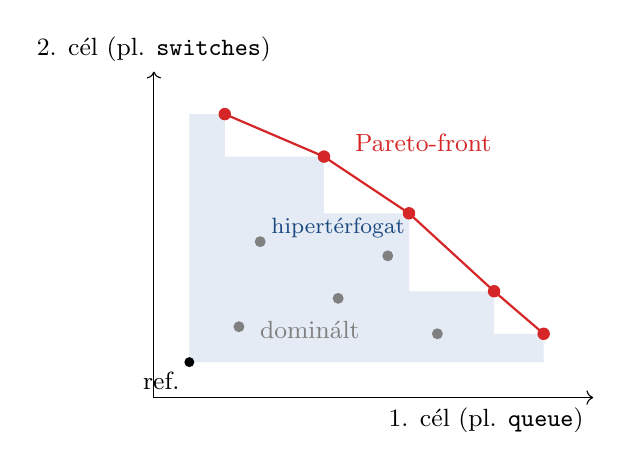
\begin{tikzpicture}[scale=0.9,font=\small]
  \draw[->] (0,0) -- (6.2,0) node[below left] {1. cél (pl. \kod{queue})};
  \draw[->] (0,0) -- (0,4.6) node[above] {2. cél (pl. \kod{switches})};
  \fill[fokek!12] (0.5,0.5) rectangle (1,4) (0.5,0.5) rectangle (2.4,3.4) (0.5,0.5) rectangle (3.6,2.6)
       (0.5,0.5) rectangle (4.8,1.5) (0.5,0.5) rectangle (5.5,0.9);
  \foreach \p in {(1,4),(2.4,3.4),(3.6,2.6),(4.8,1.5),(5.5,0.9)} \fill[piros] \p circle (2.5pt);
  \draw[piros,thick] (1,4) -- (2.4,3.4) -- (3.6,2.6) -- (4.8,1.5) -- (5.5,0.9);
  \foreach \p in {(1.5,2.2),(2.6,1.4),(3.3,2.0),(1.2,1.0),(4.0,0.9)} \fill[gray] \p circle (2.2pt);
  \fill (0.5,0.5) circle (2pt) node[below left] {ref.};
  \node[piros,right] at (2.7,3.6) {Pareto-front};
  \node[gray] at (2.2,0.95) {dominált};
  \node[fokek!80!black,align=center] at (2.6,2.4) {\footnotesize hipertérfogat};
\end{tikzpicture}
\caption{Pareto-front két maximalizálandó célra. A kék terület a hipertérfogat a referenciaponthoz
  képest: minél nagyobb, annál jobb és szerteágazóbb a front.}
\label{fig:pareto}
\end{figure}

A legtöbb RL algoritmus skalár jutalmat vár. Két egyszerű megoldás van készen:

\begin{itemize}
  \item \textbf{Lineáris skalarizálás} (\kod{LinearScalarization}): $r = \mathbf w^\top\mathbf r$
        rögzített súllyal. Különböző súlyokkal külön ágenseket tanítva a front konvex része
        feltérképezhető.
  \item \textbf{Súly-kondicionált ágens} (\kod{WeightConditioned}): minden epizódban véletlen
        súlyt sorsol, és azt a megfigyelés végére fűzi. Egyetlen háló tanulja meg az összes
        kompromisszumot; kiértékeléskor a kívánt súlyt kell megadni.
\end{itemize}

Mindkét wrapper az eredeti vektort is visszaadja az \kod{info["vector\_reward"]} alatt.

%======================================================================
\section{Munka a könyvtárral}

\subsection{Ajánlott munkafolyamat}

\begin{enumerate}
  \item \textbf{Ismerkedés}: demó, majd \kod{01\_ismerkedes.py}.
  \item \textbf{Alapvonal}: a klasszikus vezérlők kiértékelése azonos forgalmon
        (\kod{02\_baseline\_osszehasonlitas.py}).
  \item \textbf{Tanítás}: egy vagy több ágens tanítása (pl. \kod{03\_sb3\_sulyozott\_tanitas.py}).
  \item \textbf{Kiértékelés}: vektor-hozamok azonos forgalmon, Pareto-front, hipertérfogat, valós mutatók.
\end{enumerate}

\subsection{Összehasonlító vezérlők}

\begin{center}
\begin{tabularx}{\linewidth}{@{}l>{\raggedright\arraybackslash}X@{}}
\toprule
\kod{RandomPolicy} & véletlen fázis \\
\kod{FixedTimePolicy} & fix idejű, ciklikus program \\
\kod{ActuatedPolicy} & járműkövető: amíg az aktuális fázis előjelző hurkain rövid időközönként jön jármű,
  hosszabbít (legfeljebb \kod{max\_green}-ig), utána a következő olyan fázisra vált, ahol van igény \\
\kod{LongestQueuePolicy} & mohó: a legnagyobb becsült igényű fázist választja \\
\bottomrule
\end{tabularx}
\end{center}

Egy tipikus eredmény (1800~s, három véletlen forgalom átlaga):

\begin{center}
\begin{tabular}{@{}lrrrr@{}}
\toprule
vezérlő & \kod{queue} & \kod{fairness} & \kod{switches} & átl.\ álló idő [s] \\
\midrule
véletlen        & $-463$ & $-735$ & $-148$ & 59 \\
fix 30/10/15    & $-175$ & $-226$ & $-78$  & 17 \\
járműkövető     & $-136$ & $-157$ & $-121$ & 9 \\
leghosszabb sor & $-134$ & $-156$ & $-112$ & 9 \\
\bottomrule
\end{tabular}
\end{center}

Jól látszik a kompromisszum: a fix idejű program kevesebbet vált, de többet várnak a járművek.
Egy jó MORL ágensnek legalább a fix idejű programot kell vernie, és érdemes a járműkövetővel is
összevetni.

\subsection{Kiértékelés kódban}

\begin{lstlisting}
from sumo_morl import (TJunctionMOEnv, FixedTimePolicy, evaluate_policy,
                       pareto_mask, hypervolume, plot_pareto)

env = TJunctionMOEnv()
res = evaluate_policy(env, FixedTimePolicy(env, [30, 10, 15]), seeds=[0, 1, 2])
res["mean"], res["std"], res["ground_truth"]["mean_delay_per_vehicle"]
\end{lstlisting}

Egy Stable-Baselines3 modell az \kod{sb3\_policy(model)} segítségével értékelhető ki ugyanígy.
A Pareto-front a \kod{pareto\_mask}, a hipertérfogat a \kod{hypervolume}, az ábra a
\kod{plot\_pareto} függvénnyel készíthető. Különböző módszereket mindig ugyanazokkal a
\kod{seed}-ekkel és ugyanazzal a referenciaponttal hasonlíts össze.

\subsection{Tanítás Stable-Baselines3-mal}

\begin{lstlisting}
from stable_baselines3 import DQN
from sumo_morl import TJunctionMOEnv, LinearScalarization

env = LinearScalarization(TJunctionMOEnv(ground_truth=False), weights=[0.6, 0.3, 0.1])
model = DQN("MlpPolicy", env, verbose=1).learn(total_timesteps=50_000)
model.save("dqn_w06_03_01")
\end{lstlisting}

Egy egyórás epizód kb.\ 400--700 döntést jelent, és egy átlagos gépen néhány másodperc alatt fut
le. Tanításhoz érdemes a \kod{ground\_truth=False} beállítás, mert gyorsabb. Több környezet
párhuzamosan is futtatható (pl. \kod{SubprocVecEnv}), mindegyik saját SUMO-folyamatot indít.

%======================================================================
\section{Feladatötletek}

\paragraph{Bevezető}
\begin{enumerate}
  \item Futtasd a demót \kod{--gui}-val. Melyik fázisváltás a leghosszabb, és miért?
  \item Keress olyan fix idejű zöldidőket, amelyek a \kod{queue} célban jobbak az alapértelmezettnél.
        Melyik másik cél romlik közben?
\end{enumerate}

\paragraph{Egycélúból többcélúba}
\begin{enumerate}[resume]
  \item Taníts DQN-t vagy PPO-t 5--10 különböző súlyvektorral. Rajzold fel a Pareto-frontot, számold
        ki a hipertérfogatot, és vesd össze a klasszikus vezérlőkkel.
  \item Taníts egyetlen súly-kondicionált ágenst, és értékeld ki ugyanazokkal a súlyokkal. Melyik
        front jobb, és mennyivel kevesebb tanítás kellett hozzá?
  \item Definiálj saját célfüggvényt, és vizsgáld meg, hogyan változik a front.
\end{enumerate}

\paragraph{Haladó}
\begin{enumerate}[resume]
  \item Valósíts meg egy vektor-Q-értékes MORL algoritmust (pl. Envelope Q-learning).
  \item Használj nemlineáris (pl. Csebisev) skalarizálást. Találsz-e pontot a front nem konvex részén?
  \item Írj wrappert, amely a diszkontot a lépés hosszához igazítja ($\gamma^{\text{elapsed}}$).
  \item Tanítsd az ágenst alacsony forgalmon, és értékeld ki csúcsórás profillal
        (\kod{Demand.random(rng, profile=(0.5, 1, 1.5, 1))}). Mennyire robusztus?
  \item Hagyj el egy detektortípust a megfigyelésből. Melyik detektor a legfontosabb az ágensnek?
\end{enumerate}

\paragraph{Kiértékelési tanácsok}
\begin{itemize}
  \item Mindig azonos forgalmon (azonos \kod{seed}) hasonlíts össze vezérlőket.
  \item Legalább 3--5 epizód átlagát és szórását add meg.
  \item A jutalmakon kívül a valós mutatókat (\kod{info["ground\_truth"]}) is közöld.
\end{itemize}

%======================================================================
\appendix
\section{Gyakori problémák}

\begin{description}[style=nextline,leftmargin=1.5em]
  \item[\enquote{Nem található a(z) 'sumo' program}]
    Telepítsd a csomagot \kod{pip install -e .} paranccsal (ez hozza a SUMO-t), vagy állítsd be a
    \kod{SUMO\_HOME} változót a meglévő SUMO-telepítésre.
  \item[A \kod{--gui} nem nyit ablakot]
    Távoli gépen vagy Colabban nincs grafikus felület; ott a \kod{gui=False} használható.
  \item[Lassú a tanítás]
    \kod{ground\_truth=False}, rövidebb epizód (\kod{episode\_length}), párhuzamos környezetek.
  \item[\kod{RuntimeError: Előbb hívd meg a reset()-et!}]
    A \kod{step()} előtt mindig kell egy \kod{reset()}.
  \item[Egyszerre több környezet]
    Lehetséges; minden környezet saját SUMO-folyamatot indít. Használat után hívd meg az
    \kod{env.close()}-t.
\end{description}

\section{A példaprogramok}

\begin{center}
\begin{tabularx}{\linewidth}{@{}l>{\raggedright\arraybackslash}X@{}}
\toprule
\kod{00\_demo\_fix\_ido.py} & klasszikus fix idejű program, eseménynapló, jelzésterv-ábra \\
\kod{01\_ismerkedes.py} & a jelzésterv és a detektorok kiírása, véletlen ágens \\
\kod{02\_baseline\_osszehasonlitas.py} & klasszikus vezérlők azonos forgalmon, Pareto-ábra \\
\kod{03\_sb3\_sulyozott\_tanitas.py} & DQN több súlyvektorral, Pareto-front, hipertérfogat \\
\kod{04\_sajat\_celfuggveny.py} & saját célfüggvények definiálása \\
\bottomrule
\end{tabularx}
\end{center}

\end{document}
